\section{A Rotating LED Display}
This section will deal with the, perhaps, most important part of the project.
Namely, the display.
The choice of electronics components for the display is presented along with the reasoning behind each choice.
Additionally, some compromises that were made are explained.

\subsection{The Components}
The components were chosen based on a series of requirements.
These are mentioned as they become relevant in the following paragraphs.

\paragraph{LED:}
Naturally, an LED display requires LEDs.
One requirement for the display is that it should be capable of displaying simple images at a reasonable resolution.
Reaching higher resolutions can be done either by increasing the display size and moving further away, or by increasing the "pixel" density.
In this case the latter was chosen since the version of Eagle, the software used to lay out the boards used in this project, does not allow for larger than 10$\times$10 cm boards.
Increasing "pixel" density in this case means to shrink down the LEDs and position them closer to one another.
This resulted in choosing an SMD LED.
Additionally the choice was made to use an RBG variant.
Finally, the choice fell on an Osram RGB LED.
20 of these mounted on a board will constitute the display.

\subparagraph{A Smaller Footprint:}
When laying out the board, it was found that the recommended footprint of this component is far bigger than the component itself, see figure \ref{fig:recommendedfootprint}.
Using this footprint would severely limit the ability to position the LEDs as close as was intended.
The purpose of these larger pads is, while not explained in the datasheet, presumably to dissipate the heat generated by the component.
By driving the LEDs at lower currents and thereby generating less heat, it is assumed to be safe to reduce the size of the footprint.
While it may reduce the lifespan of the LEDs significantly if they run hotter than intended, it is unlikely to damage them within the time given for the project.
The footprint created for the component can be seen in figure 
\ref{fig:finalfootprint}.

\begin{figure}[H]
	\begin{subfigure}[t]{.49\linewidth}
		\centering
		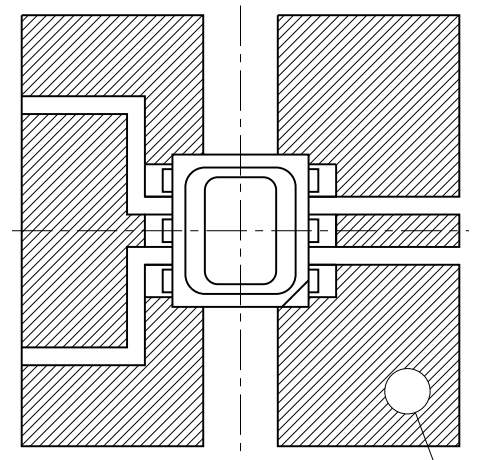
\includegraphics[width=.8\linewidth]{images/rgbfootprint}
		\caption{Recommended footprint.}
		\label{fig:recommendedfootprint}
	\end{subfigure}
	\begin{subfigure}[t]{.49\linewidth}
		\centering
		
\includegraphics[width=.8\linewidth]{images/stop}
		\caption{Reduced size footprint.}
		\label{fig:finalfootprint}
	\end{subfigure}
	\caption{Footprint of the Osram RGB LED.}
	\label{fig:footprint}
\end{figure}

\paragraph{LED Driver:}
Having 20 RGB LEDs that should all be individually controlled requires 60 control signals.
This is far more than what is available on the FPGA.
For this reason an LED driver is needed.
In order to obtain different colours it is necessary to be able to control all three channels individually. 
Additionally, in order to simplify the power supply needed, finding a version capable of 3.3v operation, as the FPGA, is a priority.
The CAT4016 chosen for this project is a constant current 16 channel LED driver.
The observant reader will notice that it has 44 channels short of what is needed.
It does, however, allow for cascading.
This means that four (or more, if need be) can be connected without requiring extra output signals from the FPGA.
It is capable of supplying up to 100 mA on each channel, far more than what is required for this application.

\subparagraph{Communicating with the CAT4016:}

As previously mentioned, this chip is capable of cascading.
This is due to the type of communication used.
The CAT4016 has a serial interface capable of running at up to 25 MHz clock speeds.
Figure \ref{fig:leddriver} shows a block diagram of the CAT4016. 
As can be seen from the diagram, this chip makes use of a shift register in order to receive its data.
The five pinouts that are concerned with communication are:

\begin{figure}[H]
	\centering
	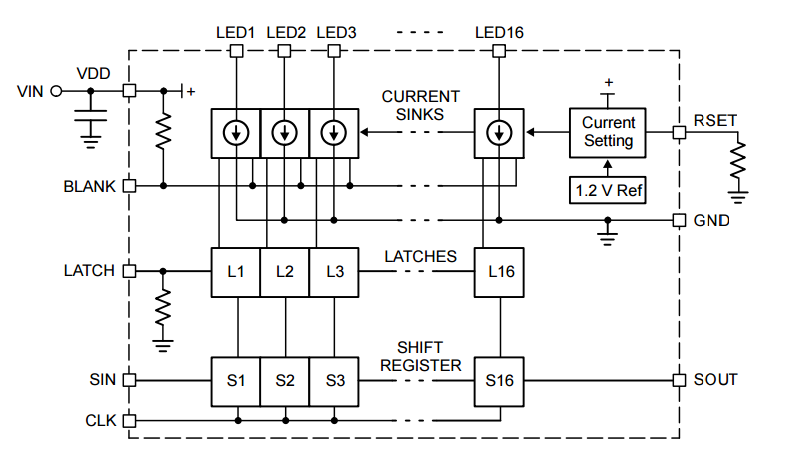
\includegraphics[width=.75\linewidth]{images/cat4016}
	\caption{Block diagram of the CAT4016 LED driver.}
	\label{fig:leddriver}
\end{figure}

\begin{itemize}
	\item \texttt{CLK:} This is the clock signal. On each rising edge of CLK data is shifted from SIN to the internal shift register.
	\item \texttt{SIN:} Serial data input. The signal on this pin is shifted into the internal shift register on each rising edge of CLK.
	\item \texttt{LATCH:} A rising edge on LATCH will cause the data in the shift registers to be output to the latches, causing the LED channels to reflect this data.
	\item \texttt{BLANK:} When pulled high, LED channels are turned off without reflecting the data in the latches. When pulled low, LED channels are turned on, reflecting the data in the latches.
	\item \texttt{SOUT:} On each rising edge on CLK the 16th bit in the shift register is made available on this pin.
\end{itemize}

\texttt{SOUT} is the reason the CAT4016 can be cascaded.
By connecting \texttt{SOUT} of one chip to \texttt{SIN} of the next, the shift register is effectively doubled.
\texttt{BLANK}, \texttt{LATCH} and \texttt{CLK} are all connected to the same signals from the FPGA.
A view of this can be seen in figure \ref{fig:simpledriver}.
Cascading four of these means that each cycle requires 64 clock cycles before \texttt{LATCH} can be pulled high.
At 25 MHz this is an update frequency of about 390 kHz.
An overview of the method used for generating a 1 kHz PWM for the LEDs can be seen in figure \ref{fig:pwmsequence}. 
Here, each cycle of the PWM is split into 100 time slices.
During each slice a new packet of 64 bits is clocked into the shift register.
Each bit in a packet represents the state of its corresponding channel at that time.
This scheme can be seen in figure \ref{fig:bitone}.
If the first bit in the first 25 sequences is high, then the duty cycle of channel 64 will be 25\%.
Notice that bit 0 corresponds to channel 64 and vice versa.
Using this technique allows for 1\% resolution on the PWM duty cycle.


\begin{figure}[H]
	\centering
	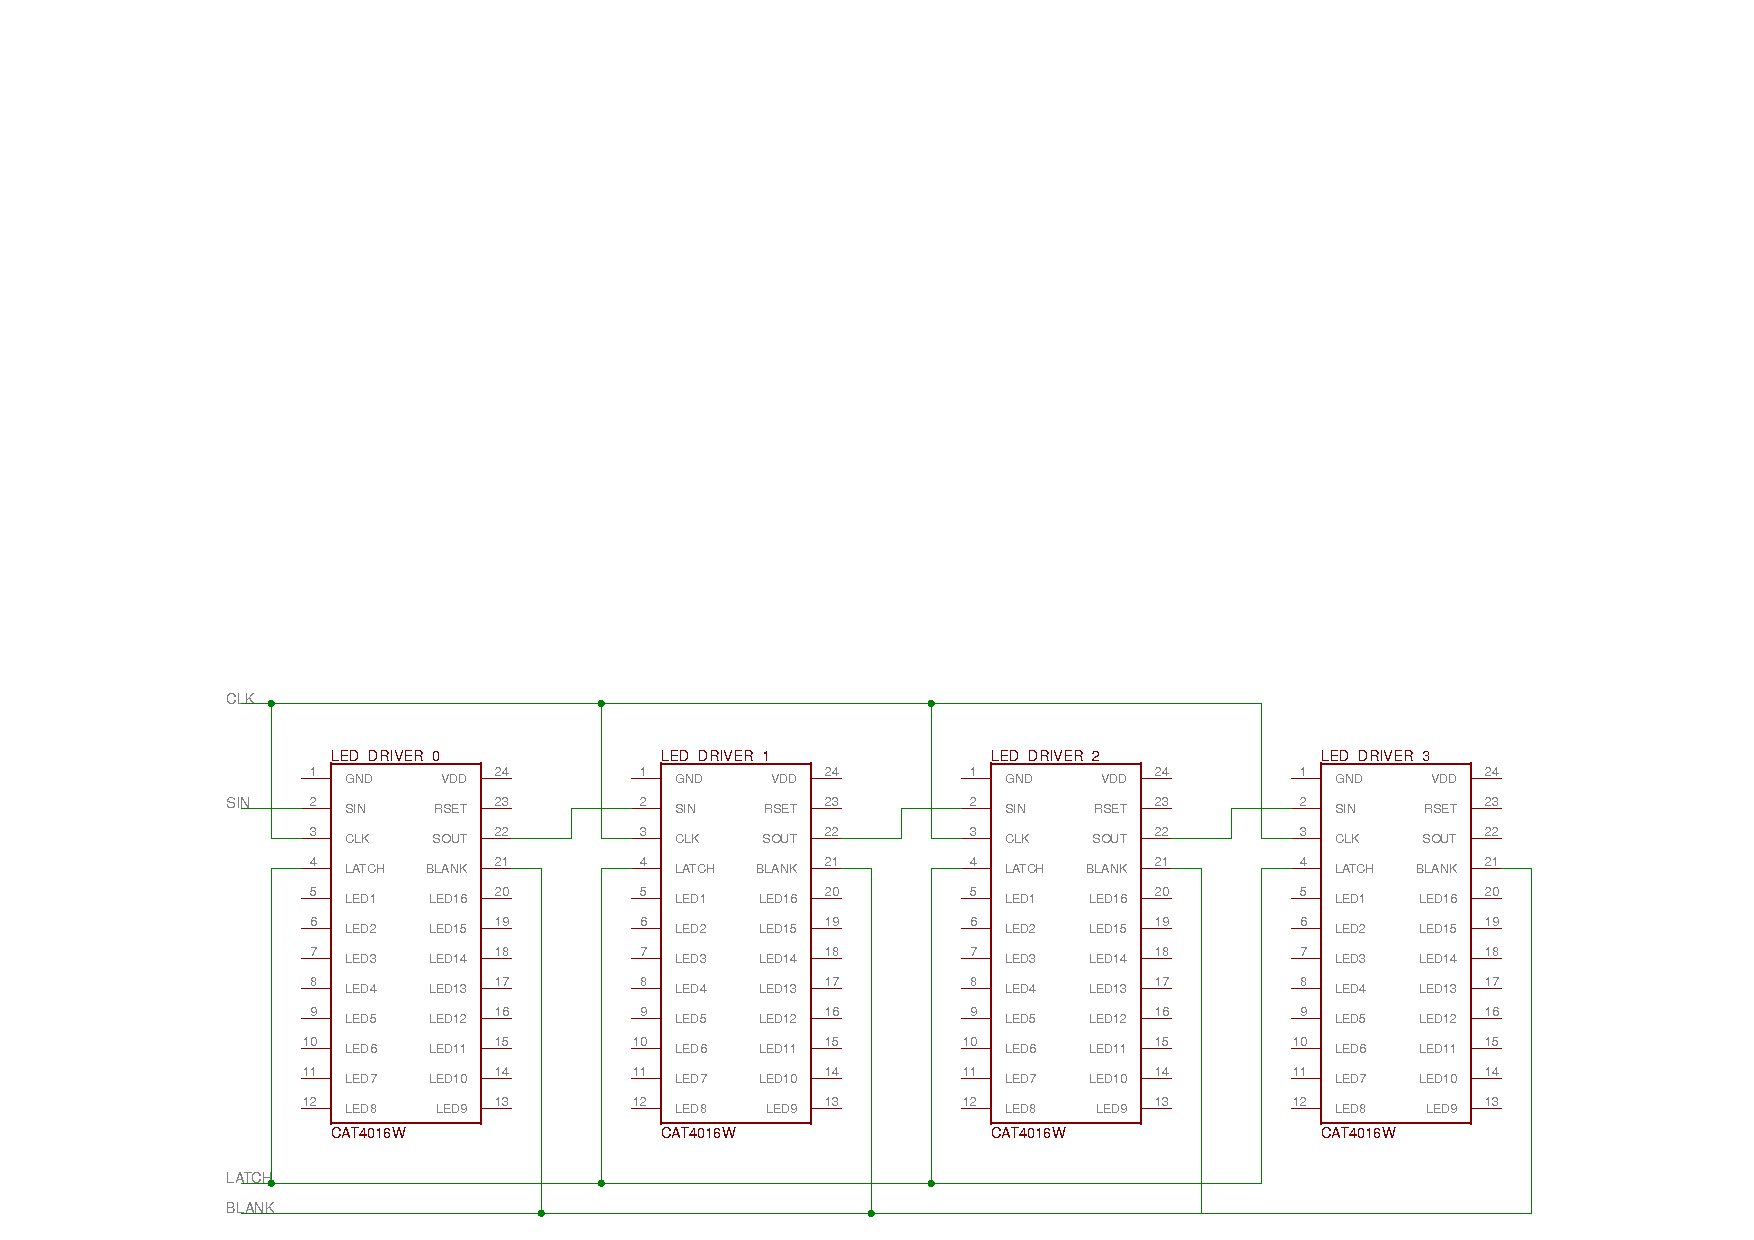
\includegraphics[width=\linewidth,trim={0 0 0 11.5cm},clip]{images/simpledriver}
	\caption{A view of four cascaded CAT4016.}
	\label{fig:simpledriver}
\end{figure}

\begin{figure}[H]
	\begin{subfigure}[t]{.49\linewidth}
		\centering
		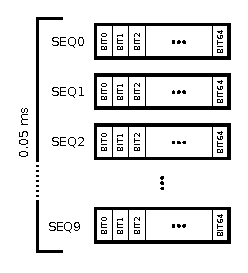
\includegraphics[width=.65\linewidth]{images/bit64}
		\caption{The complete sequence of packages sent for one cycle.}
		\label{fig:bit64}
	\end{subfigure}
	\begin{subfigure}[t]{.49\linewidth}
		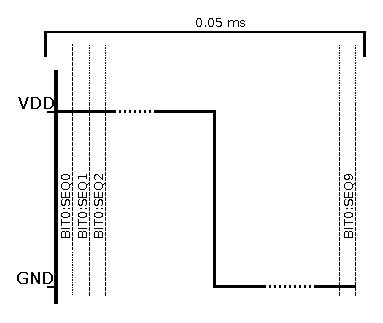
\includegraphics[width=\linewidth]{images/bitonegraph}
		\caption{Resulting signal for one channel.}
		\label{fig:bitone}
	\end{subfigure}
	\caption{Generation of the 1 kHz PWM signal used to drive the LEDs.}
	\label{fig:pwmsequence}
\end{figure}

\subparagraph{Choice of Current:}
The CAT4016 is a constant current driver.
This means that it can be set to always source a certain current.
In this case it is capable of sourcing 2 mA to 100 mA to each channel.
Setting this current is done by applying a resistor to ground on \texttt{RSET}.
The current will the follow:

$$\text{LED current} = 50 \cdot \frac{1.2}{\text{R}_\text{SET}}$$

As per the datasheet of the LEDs they do not have the same requirement for each channel, RGB.
Three options to deal with this were considered; 
first: Disregard. Since colour accuracy is not critical, it may be acceptable that some colours are more prominent than others.
Second: Sorting. The red and blue diodes of the LEDs require the same amount of current.
Only the green diode has a higher current requirement.
By driving the green diodes from the same driver, the current for these could be set independently from the rest.
Using this technique would increase complexity on the FPGA.
Third: By setting the current equal to the highest requirement set by the LED, resistors could be set in series with the other LEDs in order to limit current.
Unfortunately, due to time constraints, it was not possible to determine which method would be best suited for this project.

\paragraph{Motor:}
In order to actually have a rotating display, it is necessary to somehow rotate the display.
This is done, for the sake of simplicity, using a simple DC motor.
A motor was chosen such that it could be driven from a 12 V supply.
This would allow for reusing the power supply from the Lego Brick Sorter.
The motor chosen is the Como Drills RE540.
The power supply however, is rated only for 1 A continuous operation whereas this motor is rated
A, rather significant, detail that was not considered when ordering the components.
